\documentclass[11pt]{article}
\usepackage[utf8]{inputenc}
\usepackage[spanish]{babel}
\usepackage{amsmath}       % para las ecuaciones
\usepackage{graphicx}      % para insertar imágenes
\usepackage{listings}      % para mostrar código
\usepackage{xcolor}
\usepackage{geometry}
\usepackage{float}
\geometry{margin=2.5cm}

\lstset{
    language=Python,
    basicstyle=\ttfamily\small,
    keywordstyle=\color{blue},
    commentstyle=\color{gray},
    stringstyle=\color{orange},
    breaklines=true,
    frame=single,
    numbers=left
}

\title{
    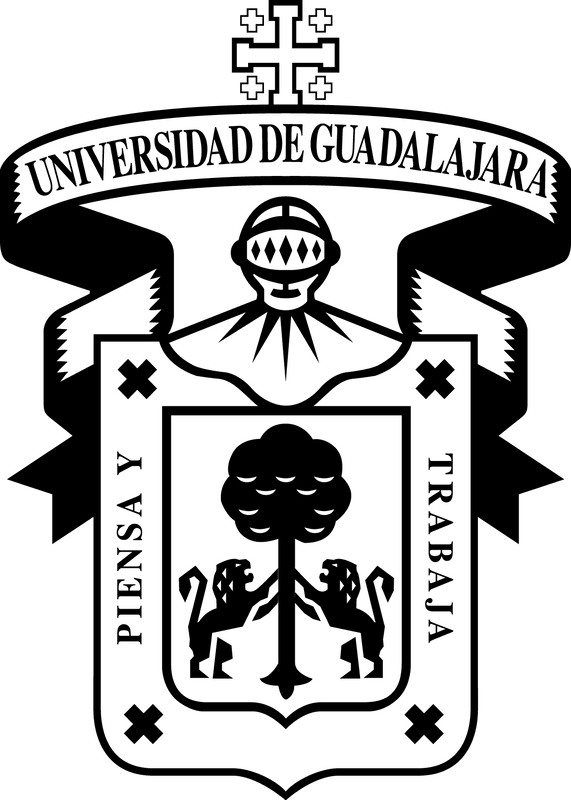
\includegraphics[width=4cm]{logo_udg.png}\\[1cm]
    A02 - Regresión Lineal: Gradiente Descendente y Pseudoinversa\\
    
    \large Algoritmos Metaheurísticos
}
\author{Jose Luis Chavez Gomez}
\date{\today}

\begin{document}
\maketitle

\section{Marco Teórico}

\subsection{Función Objetivo}
En regresión lineal multivariable, el modelo predice:
\begin{equation}
    \hat{y} = X\theta
\end{equation}

La función de costo (error cuadrático medio) es:
\begin{equation}
    J(\theta) = \frac{1}{2m}\sum_{i=1}^{m}(h_\theta(x^{(i)}) - y^{(i)})^2 = \frac{1}{2m}\|X\theta - y\|^2
\end{equation}

\subsection{Ecuaciones de Actualización de Gradiente Descendente}
El gradiente de $J(\theta)$ es:
\begin{equation}
    \nabla J(\theta) = \frac{1}{m}X^T(X\theta - y)
\end{equation}

La regla de actualización iterativa:
\begin{equation}
    \theta := \theta - \alpha \cdot \frac{1}{m}X^T(X\theta - y)
\end{equation}

\subsection{Pseudoinversa}
Igualando el gradiente a cero se obtiene la ecuación normal:
\begin{equation}
    \theta = (X^TX)^{-1}X^Ty = X^+y
\end{equation}

Esta solución analítica evita el proceso iterativo de gradiente descendente, resolviendo directamente el sistema de ecuaciones normales mediante la pseudoinversa de Moore-Penrose, la cual generaliza el concepto de matriz inversa incluso cuando $X^TX$ no es invertible.

\section{Implementación}

\subsection{Generación de Datos (dataset.py)}

\begin{lstlisting}
import numpy as np

def generar_datos(m=100, n=2, seed=42):
    np.random.seed(seed)
    X_raw = np.random.rand(m, n) * 10
    X = np.hstack([np.ones((m, 1)), X_raw])
    theta_real = np.array([5, 2, -3])
    ruido = np.random.randn(m) * 1.0
    y = X @ theta_real + ruido

    return X, y, theta_real
\end{lstlisting}

Se generan $m=100$ ejemplos con $n=2$ variables independientes, más una columna de unos para el término de sesgo (bias). Los valores objetivo $y$ se construyen a partir de un $\theta_{real} = [5, 2, -3]$ conocido, agregando ruido gaussiano para simular condiciones realistas.

\subsection{Gradiente Descendente (gradient\_descent.py)}

\begin{lstlisting}
import numpy as np
import matplotlib.pyplot as plt
from dataset import generar_datos

def objective_function(X, y, theta):
    m = len(y)
    J_theta = (np.sum((X @ theta - y) ** 2)) / (2*m)
    return J_theta

def gradient_descent(X, y, theta_inicial, alpha, iteraciones):
    m = len(y)
    costos = []
    theta = theta_inicial
    for i in range(iteraciones):
        gradiente = (1/m) * X.T @ (X @ theta - y)
        theta = theta - alpha * gradiente
        costos.append(objective_function(X, y, theta))
    return theta, costos

if __name__ == "__main__":
    X, y, theta_real = generar_datos()

    costo = objective_function(X, y, theta_real)
    print("Costo con theta_real:", costo)

    theta_prueba = np.zeros(3)
    costo_malo = objective_function(X, y, theta_prueba)
    print("Costo con theta en ceros: ", costo_malo)

    theta_inicial = np.zeros(3)
    theta_final, costos = gradient_descent(X, y, theta_inicial, alpha=0.01, iteraciones=10000)

    print("Theta final:", theta_final)
    print("Theta real:", theta_real)
    print("Último costo:", costos[-1])
    plt.plot(costos)
    plt.xlabel("Iteración")
    plt.ylabel("J(theta)")
    plt.title("Convergencia de Gradiente Descendente")
    plt.savefig("convergencia_gd.png")
    plt.show()
\end{lstlisting}

\subsection{Pseudoinversa (pseudoinverse.py)}
\begin{lstlisting}
import numpy as np
from dataset import generar_datos
from gradient_descent import objective_function

def pseudoinversa(X, y):
    theta = np.linalg.pinv(X) @ y
    return theta

if __name__ == "__main__":
    X, y, theta_real = generar_datos()

    theta_pinv = pseudoinversa(X, y)
    print("Theta pseudoinversa:", theta_pinv)
    print("Theta real:", theta_real)

    costo_pinv = objective_function(X, y, theta_pinv)
    print("Costo con pseudoinversa:", costo_pinv)
\end{lstlisting}

\subsection{Comparación (compare.py)}
\begin{lstlisting}
from dataset import generar_datos
from gradient_descent import gradient_descent, objective_function
from pseudoinverse import pseudoinversa
import numpy as np
import matplotlib.pyplot as plt

X, y, theta_real = generar_datos()

theta_gd, costos = gradient_descent(X, y, np.zeros(3), alpha=0.01, iteraciones=10000)
theta_pinv = pseudoinversa(X, y)
costo_pinv = objective_function(X, y, theta_pinv)

plt.plot(costos, label="Gradiente Descendente")
plt.axhline(y=costo_pinv, color='r', linestyle='--', label="Pseudoinversa (óptimo)")
plt.xlabel("Iteración")
plt.ylabel("J(theta)")
plt.title("Convergencia de GD vs. Pseudoinversa")
plt.legend()
plt.savefig("comparacion_gd_pinv.png")
plt.show()
\end{lstlisting}

Este script integra ambos métodos utilizando exactamente el mismo conjunto de datos, permitiendo comparar de forma justa el costo final alcanzado por cada uno.

\section{Resultados}

\subsection{Experimento: Gradiente Descendente}

Antes de ejecutar el algoritmo, se evaluó la función de costo con dos valores de referencia. Con $\theta_{real} = [5, 2, -3]$ (los parámetros usados para generar los datos sintéticos) se obtuvo $J(\theta) = 0.5065$, un valor cercano a la varianza del ruido gaussiano introducido, como es esperado. Con $\theta = [0, 0, 0]$ se obtuvo $J(\theta) = 57.0098$, confirmando que la función de costo distingue correctamente entre un modelo bien ajustado y uno arbitrario.

Tras ejecutar gradiente descendente con $\alpha = 0.01$ durante 10{,}000 iteraciones, se obtuvo:
\begin{equation}
    \theta_{GD} = [4.772,\ 2.034,\ -2.965], \quad J(\theta_{GD}) = 0.4907
\end{equation}

\begin{figure}[H]
    \centering
    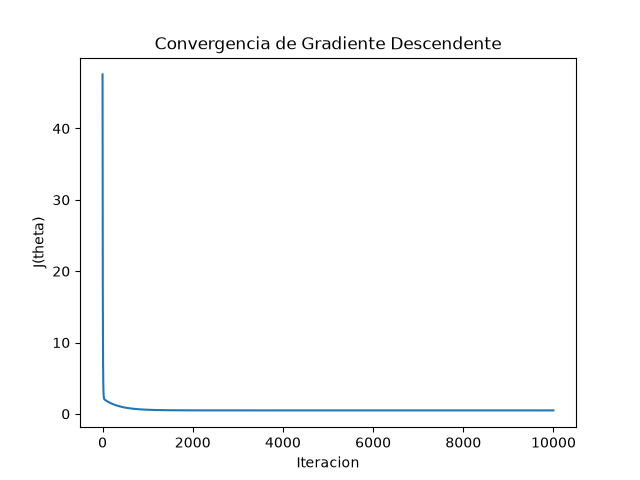
\includegraphics[width=0.6\textwidth]{convergencia_gd.png}
    \caption{Convergencia del costo J(theta) a lo largo de las iteraciones}
\end{figure}

Como se observa en la Figura 1, el costo desciende abruptamente durante las primeras iteraciones y después se estabiliza, indicando que el algoritmo convergió correctamente antes de alcanzar las 10{,}000 iteraciones.

\subsection{Experimento: Pseudoinversa}

Al resolver el problema mediante la ecuación normal (pseudoinversa), se obtuvo:
\begin{equation}
    \theta_{pinv} = [4.772,\ 2.034,\ -2.965], \quad J(\theta_{pinv}) = 0.4907
\end{equation}

Este resultado se obtiene en una sola operación matricial, sin necesidad de iterar ni de elegir una tasa de aprendizaje $\alpha$.

\subsection{Comparación}

\begin{table}[h]
\centering
\begin{tabular}{lccc}
\hline
\textbf{Método} & \textbf{$\theta_0$ (bias)} & \textbf{$\theta_1$} & \textbf{$\theta_2$} \\
\hline
$\theta_{real}$ & 5.000 & 2.000 & -3.000 \\
Gradiente Descendente & 4.772 & 2.034 & -2.965 \\
Pseudoinversa & 4.772 & 2.034 & -2.965 \\
\hline
\end{tabular}
\caption{Comparación de parámetros obtenidos por cada método}
\end{table}

\begin{table}[h]
\centering
\begin{tabular}{lc}
\hline
\textbf{Método} & \textbf{$J(\theta)$} \\
\hline
$\theta_{real}$ & 0.5065 \\
$\theta = [0,0,0]$ & 57.0098 \\
Gradiente Descendente & 0.4907 \\
Pseudoinversa & 0.4907 \\
\hline
\end{tabular}
\caption{Costo obtenido por cada método}
\end{table}

Es importante notar que ambos métodos convergen a un valor ligeramente distinto de $\theta_{real}$. Esto no representa un error, sino el comportamiento esperado: debido al ruido aleatorio agregado a los datos, el óptimo \textit{muestral} (el mejor $\theta$ para esta muestra específica) no coincide exactamente con el $\theta_{real}$ usado para generarla. El hecho de que gradiente descendente y pseudoinversa converjan prácticamente al mismo valor confirma que ambos algoritmos encontraron correctamente ese óptimo.

\begin{figure}[H]
    \centering
    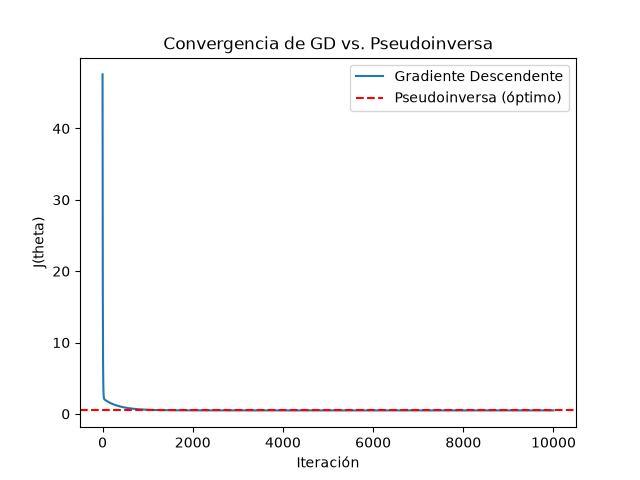
\includegraphics[width=0.7\textwidth]{comparacion_gd_pinv.png}
    \caption{Comparación entre GD y la solución de la pseudoinversa}
\end{figure}

En la Figura 2 se observa cómo la curva de convergencia de gradiente descendente se aproxima asintóticamente a la línea horizontal que representa el costo óptimo obtenido mediante la pseudoinversa, evidenciando que ambos métodos convergen a la misma solución.

\section{Conclusión}

Se implementaron dos enfoques para resolver el problema de regresión lineal multivariable: un método iterativo (gradiente descendente) y un método analítico directo (pseudoinversa). Ambos métodos convergieron prácticamente al mismo valor de $\theta$ y al mismo costo final ($J(\theta) \approx 0.4907$), validando la correctitud de ambas implementaciones.

La principal diferencia observada entre ambos métodos es de naturaleza conceptual: gradiente descendente requiere elegir una tasa de aprendizaje $\alpha$ y un número de iteraciones, y su convergencia es progresiva, mientras que la pseudoinversa resuelve el problema en una sola operación matricial sin parámetros que ajustar. Sin embargo, esta ventaja de la pseudoinversa depende de que el problema sea lineal y de tamaño manejable, ya que el cálculo de $(X^TX)^{-1}$ o de la pseudoinversa puede volverse computacionalmente costoso para conjuntos de datos muy grandes o con muchas variables, escenario en el cual gradiente descendente resulta más práctico a pesar de su naturaleza iterativa.

\section {Referencias}
\begin{itemize}
    \item[] Géron, A. (2022). \textit{Hands-on machine learning with Scikit-Learn, Keras, and TensorFlow: Concepts, tools, and techniques to build intelligent systems} (3rd ed.). O'Reilly Media.

    \item[] Goodfellow, I., Bengio, Y., \& Courville, A. (2016). \textit{Deep learning}. MIT Press.

    \item[] Strang, G. (2016). \textit{Introduction to linear algebra} (5th ed.). Wellesley-Cambridge Press.
\end{itemize}

\end{document}